\documentclass[12pt,a4paper]{article}
\usepackage{fontspec}
\defaultfontfeatures{Ligatures=TeX}
\usepackage{graphicx,textcomp}
\usepackage{amsmath,amssymb,float,caption,xcolor,hyperref,fancyhdr}
\usepackage{geometry,booktabs,array}
\geometry{margin=1in}
\setlength{\headheight}{14.5pt}
\pagestyle{fancy}\fancyhf{}\lhead{Automatic GFL$\leftrightarrow$GFM Switching via AGSI (two IBRs)}\rhead{\thepage}
\hypersetup{colorlinks=true,linkcolor=blue,urlcolor=blue,citecolor=blue}
\renewcommand{\arraystretch}{1.12}
\linespread{1.08}

\title{\textbf{Automatic Grid-Following $\leftrightarrow$ Grid-Forming Mode Switching of Two IBRs
via an Adaptive Grid Stability Index (AGSI) on an Infinite Bus}\\
\large Principle, switching equation, and current-continuous (bumpless) transfer}
\date{23 July 2026}

\begin{document}
\maketitle

\begin{abstract}
This report (separate from the earlier 6-state GFL/GFM comparison report) presents the
\textbf{automatic mode-switching supervisor} that toggles two IBRs between grid-following (GFL) and
grid-forming (GFM) on a common point of connection (PCC) behind one line to an ideal infinite bus. The
decision uses a \emph{single index equation}, the \textbf{Adaptive Grid Stability Index (AGSI)}
(EECON49-P4 guideline), compared with two \emph{reference lines} ($\Gamma_{on},\Gamma_{off}$) plus a
hysteresis band and dwell times. A temporary weak-grid event drives the AGSI of both units up to
$\Gamma_{on}$ (switch GFL$\to$GFM); on recovery the AGSI falls below $\Gamma_{off}$ (switch back
GFM$\to$GFL). Every transfer is \emph{current-continuous} (bumpless). Project-owned time-domain
simulation (no external solver) confirms a converged bidirectional cycle, current continuity at the
$10^{-17}$ level, and passing automated tests. All equations and thresholds are traceable; nothing was
tuned to bias the result.
\end{abstract}

\section{Scope and link to the previous report}
The previous report (\texttt{report\_ibr\_gfl\_gfm\_en}) documented the two reduced 6-state IBR models
(GFL, GFM) and their SSSA. Here those models are \emph{reused as the single source of truth} for the
branch equations, and a \textbf{supervisor} that switches modes automatically is added. Source
discipline: the switching structure (AGSI, thresholds, dwell) follows the EECON49-P4 strategy
\cite{eecon49en} as a \emph{design guideline, not an exact reproduction} (the paper's Bayesian
Optimization is not used here); classification \texttt{PROJECT\_DERIVED\_SOURCE\_GUIDED}. Bidirectional
switching and state transfer are consistent with the switchable-control literature
\cite{ding2025e,liu2024e,gao2025e}.

\section{Principle and test system}
GFL relies on a PLL and is well behaved in strong grids but loses damping / stability in weak grids;
GFM forms its own voltage/frequency reference and rides through weak grids. The supervisor therefore
switches GFL$\to$GFM when the system is stressed and GFM$\to$GFL when it recovers. \textbf{The disturbance
that forces the switch} here is a temporary \emph{grid-weakening event}: at $t_{ev}$ the line impedance to
the infinite bus is multiplied ($\times4$ default, $Z_{line}:0.30j\!\to\!1.20j$), i.e.\ the SCR drops to
$\sim1/4$ (modelling loss of a strong transmission path); the framework also supports a $V_\infty$
phase/voltage step and loss of reference ($\mathrm{GRA}=0$, islanding). Causal chain: a GFL is a current
source, so through the high-impedance line the PCC voltage sags ($|V|:0.99\!\to\!0.79$), which sharply
raises $J_V$; near the max-power (voltage-collapse) nose the PLL loses damping, adding $J_f,J_R$; the
weighted AGSI then crosses $\Gamma_{on}$ and the units switch to GFM (which forms voltage + virtual
inertia and rides through the weak grid). On line restoration the grid is strong again, AGSI falls below
$\Gamma_{off}$, and the units return to GFL. Two IBRs start as GFL
at a common PCC; the PCC algebraic balance is
\begin{equation}
I_1(x_1,V) + I_2(x_2,V) = \frac{V - V_\infty}{Z_{line}}.
\end{equation}
Each device is an object (\texttt{ibr.SwitchableIbr6}) wrapping both 6-state branches; the active state
dimension is always 6, and a switch re-initialises those 6 slots to the target-branch equilibrium.

\section{The switching equation (AGSI) and how the index acts}
The AGSI merges four normalised PCC deviations into one dimensionless index:
\begin{equation}
\mathrm{AGSI} = w_V J_V + w_f J_f + w_R J_R + w_P J_P,\qquad w_V+w_f+w_R+w_P=1,
\end{equation}
\begin{equation}
J_V=\frac{|V-V_{ref}|}{\Delta V_{base}},\quad
J_f=\frac{|f-f_0|}{\Delta f_{base}},\quad
J_R=\frac{|\mathrm{d}f/\mathrm{d}t|}{\Delta\mathrm{RoCoF}_{base}},\quad
J_P=\frac{|P_{ref}-P|}{\Delta P_{base}}.
\end{equation}
In GFL $f$ is the PLL frequency; in GFM it is the VSG rotor frequency; $\mathrm{d}f/\mathrm{d}t$ is a
one-per-step numerical RoCoF. Each term is a different ``stress view'' of the PCC:
\begin{itemize}\itemsep2pt
\item $J_V$ --- \textbf{voltage deviation}: $V$ = measured PCC voltage vs nominal $V_{ref}=1$ pu; a weak
grid / heavy loading sags $V$ (the dominant driver here). $\Delta V_{base}=0.10$ pu ($10\%\Rightarrow J_V=1$).
\item $J_f$ --- \textbf{frequency deviation}: how far $f$ strays from $f_0=60$ Hz; indicates power
imbalance / loss-of-synchronism tendency. $\Delta f_{base}=0.50$ Hz.
\item $J_R$ --- \textbf{RoCoF}: rate of change of frequency, a standard low-inertia stability metric
\cite{entsoe_rocof2}; large RoCoF $\Rightarrow$ low effective inertia $\Rightarrow$ favour GFM (virtual
inertia). $\Delta\mathrm{RoCoF}_{base}=1.0$ Hz/s (grid-code scale $\sim$0.5--2 Hz/s).
\item $J_P$ --- \textbf{active-power tracking error}: commanded $P_{ref}$ vs delivered $P$; a large error
means the converter cannot meet its command (weak grid / current limit). $\Delta P_{base}=0.20$ pu.
\item weights $w_\bullet$ (sum 1) set the relative importance; the normalisation bases make the terms
dimensionless and comparable (a deviation equal to its base gives sub-index 1); $\Gamma_{on}/\Gamma_{off}$
are the AGSI thresholds; $\mathrm{GRA}$ flags whether a voltage/frequency reference exists; $T_d$ is the
dwell that rejects momentary spikes.
\end{itemize}
With grid-reference availability $\mathrm{GRA}\in\{0,1\}$ the logic is:
\begin{align}
\text{GFL}\to\text{GFM}:&\quad (\mathrm{AGSI}\ge\Gamma_{on})\lor(\mathrm{GRA}=0)\ \text{held}\ \ge T_{d,on},\\
\text{GFM}\to\text{GFL}:&\quad (\mathrm{AGSI}<\Gamma_{off})\land(\mathrm{GRA}=1)\ \text{held}\ \ge T_{d,off}.
\end{align}
Since $\Gamma_{on}>\Gamma_{off}$, the band $[\Gamma_{off},\Gamma_{on}]$ is a \emph{hysteresis} region
with no switching; the dwell times reject momentary transients (e.g.\ a brief RoCoF spike at a topology
change). Defaults (EECON49-P4 \S4.1 guideline): $w=[0.30,0.30,0.25,0.15]$;
$\Delta V_{base}=0.10$ pu, $\Delta f_{base}=0.50$ Hz, $\Delta\mathrm{RoCoF}_{base}=1.0$ Hz/s,
$\Delta P_{base}=0.20$ pu; $\Gamma_{on}=0.65$, $\Gamma_{off}=0.35$; $T_{d,on}=0.10$ s,
$T_{d,off}=1.00$ s.

\begin{figure}[H]\centering
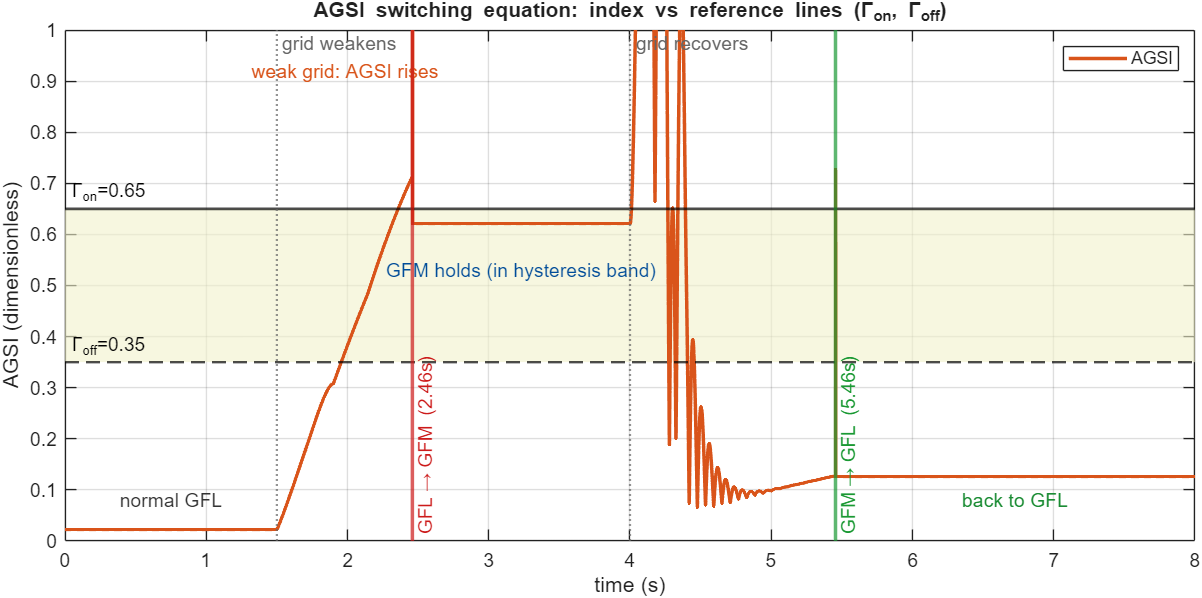
\includegraphics[width=\textwidth]{figures/two_ibr_switch/agsi_annotated.png}
\caption{AGSI versus the two reference lines (yellow = hysteresis band). The index rises to
$\Gamma_{on}$ (switch to GFM, red), holds in the band while the grid is weak, then falls below
$\Gamma_{off}$ after recovery (switch back to GFL, green).}
\label{fig:agsi_en}
\end{figure}

\section{Bumpless transfer}
At the switch instant, the terminal $(V,P,Q)$ is read from the active injection and the target branch is
initialised to the equilibrium delivering the same $(P,Q)$ at the same $V$. Because both branches give
$I=\overline{(P+jQ)/V}$, the injected current is continuous ($|I^+-I^-|\approx2.8\times10^{-17}$ in both
directions). The GFM references are back-solved so its swing/voltage derivatives are also zero at the
instant.

\section{Results}
Figure~\ref{fig:overview_en} shows the default scenario (line weakened $\times4$ over $1.5$--$4.0$ s,
smooth $0.4$ s ramp, no phase snap): normal GFL $\to$ AGSI rises $\to$ GFL$\to$GFM at $\approx2.46$ s
$\to$ GFM holds the weak grid (AGSI in the hysteresis band) $\to$ grid recovers $\to$ GFM$\to$GFL at
$\approx5.45$ s $\to$ normal GFL. Verified: two transitions per unit ending in GFL; Newton converges at
every step; current continuous to $\sim10^{-17}$; frequency swing only $\pm0.6$ Hz; pre-event
equilibrium residual at machine precision; all tests in \texttt{tests/test\_ibr\_switchable6.m} pass
(including the \texttt{solve\_case} route).

\begin{figure}[H]\centering
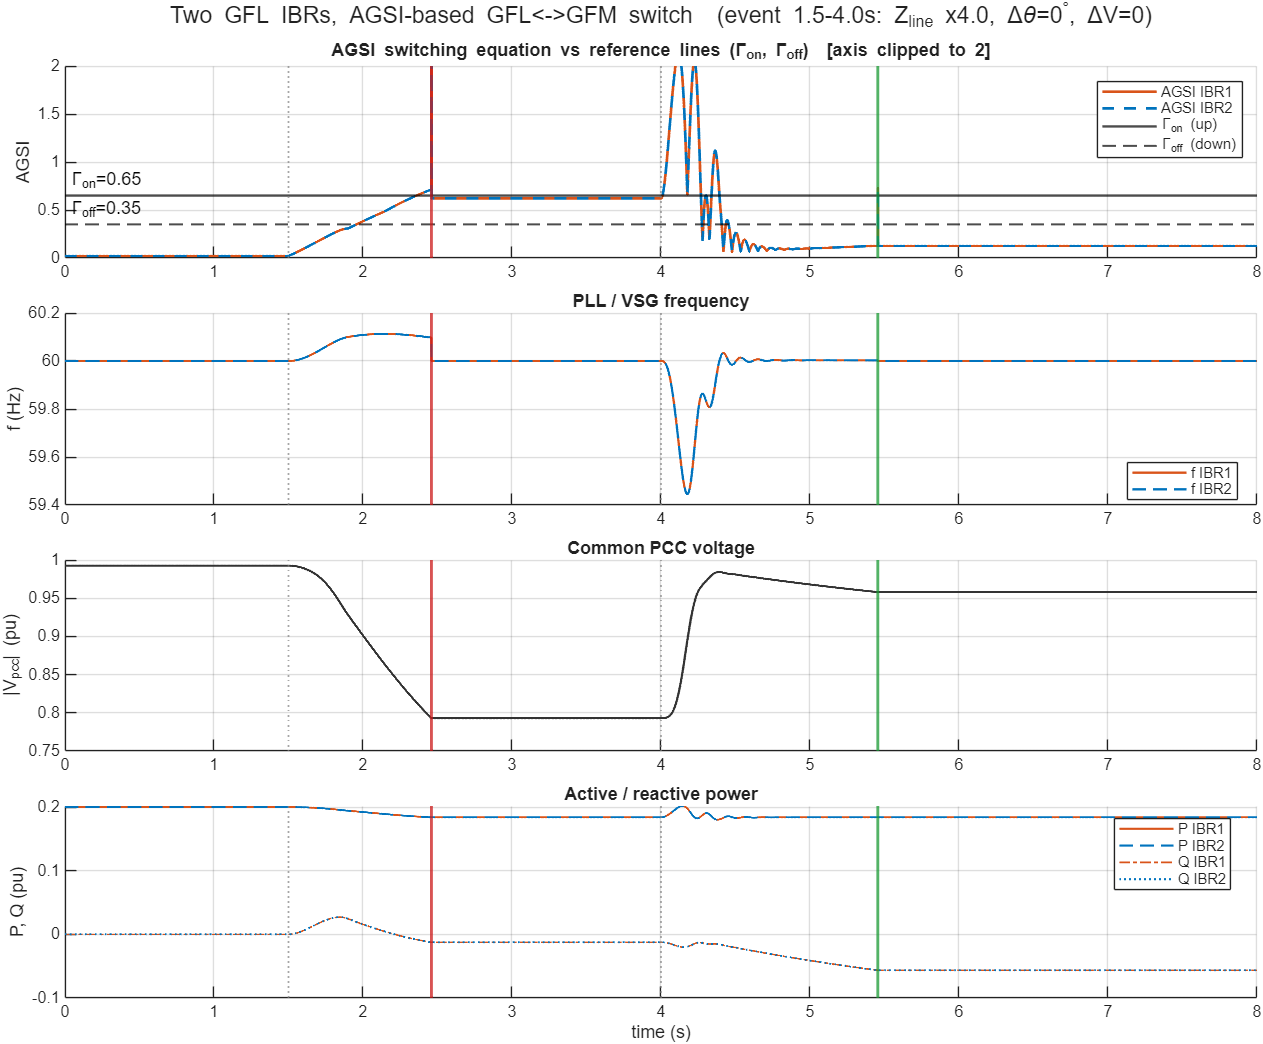
\includegraphics[width=\textwidth]{figures/two_ibr_switch/switch_overview.png}
\caption{Four-panel overview: AGSI vs reference lines (red = GFL$\to$GFM, green = GFM$\to$GFL),
PLL/VSG frequency, PCC voltage, and $P,Q$ of both IBRs.}
\label{fig:overview_en}
\end{figure}

\section{How to run}
\texttt{run\_two\_ibr\_switch} (opens a settings dialog, then runs) \textbullet\
\texttt{run\_two\_ibr\_switch(Zline\_factor=5)} (skip the dialog) \textbullet\
\texttt{solve\_case('analysis','ibr','case','two\_ibr\_switch')}.

\section{Limitations}
Weights/thresholds are \texttt{PROJECT\_DERIVED\_SOURCE\_GUIDED} (no Bayesian Optimization); at a common
PCC both IBRs see the same voltage and switch together (a separate-bus network is the next step); the
driver is a diagnostic, not a production TS kernel; no current limiter/LVRT. The result is structural
evidence of the switching mechanism, not a fault-ride-through certification.

\clearpage
\section{Extended study: automatic switching on two multi-machine systems}
This section extends the single-PCC demonstration to two multi-machine systems in which one
synchronous generator (SG) shares the network with several grid-following (GFL) IBRs. On an SG
trip the stressed IBRs form (GFL$\to$GFM) to hold the island; on a synchronised SG reclose the
SG re-takes the slack and the IBRs hand the reference back. The decision uses the same AGSI
supervisor, upgraded here to \textbf{AGSI++}.

\subsection{AGSI / AGSI++ switching index (corrected)}
The Adaptive Grid-Support Index is a weighted sum of normalised sub-indices, evaluated per IBR
every step:
\begin{align}
J_V &= \frac{|V-V_{ref}|}{\Delta V_{base}}, &
J_f &= \frac{|f-f_0|}{\Delta f_{base}},\\
J_R &= \frac{|\mathrm{d}f/\mathrm{d}t|}{\Delta R_{base}}, &
J_P &= \frac{|P_{ref}-P|}{\Delta P_{base}},\\
J_{SCR} &= \max\!\Big(0,\ \tfrac{SCR_{crit}}{SCR}-1\Big), &
J_{lock} &= \frac{|v_q|}{\Delta v_{q,base}}.
\end{align}
with $\Delta V_{base}=0.10$ pu, $V_{ref}=1.0$; $\Delta f_{base}=0.50$ Hz, $f_0=60$;
$\Delta R_{base}=1.0$ Hz/s (RoCoF); $\Delta P_{base}=0.20$ pu; $SCR_{crit}=3$; and
$\Delta v_{q,base}=0.10$. The composite index is
\begin{equation}
\mathrm{AGSI}=w_V J_V + w_f J_f + w_R J_R + w_P J_P + w_{SCR}J_{SCR} + w_{lock}J_{lock}.
\end{equation}
Plain AGSI uses $[w_V,w_f,w_R,w_P]=[0.30,0.30,0.25,0.15]$ (with $w_{SCR}=w_{lock}=0$); AGSI++
uses $[0.25,0.25,0.15,0.10,0.15,0.10]$ (sum $=1$). Switching applies hysteresis and dwell:
\begin{align}
\text{GFL}\to\text{GFM}:&\quad \mathrm{AGSI}\ge\Gamma_{on}=0.65\ \text{held for}\ \ge T_{d,on},\\
\text{GFM}\to\text{GFL}:&\quad \mathrm{AGSI}<\Gamma_{off}=0.35\ \text{held for}\ \ge T_{d,off}.
\end{align}
AGSI++ low-pass filters the RoCoF term ($\tau_R=0.05$ s) to reject the one-sample RoCoF spike
that causes no-dwell chattering, and adds $J_{SCR}$ (weak-grid strength) and $J_{lock}$ (a PLL
loss-of-lock proxy using $|v_q|$).

\subsection{Reduced-6 IBR models (state order + equations)}
Each functional block contributes two dynamic states; the input is $u=[P_{ref};Q_{ref}]$ on
system base. \textbf{GFL (grid-following)} has state order
$x=[\,i_d,\ i_q,\ \delta_{\mathrm{PLL}},\ \xi_{\mathrm{PLL}},\ \xi_P,\ \xi_Q\,]$ (dq L-filter
currents on inverter base, SRF-PLL angle and PI integrator, and the $P$/$Q$ outer-PI integrators):
\begin{align}
\dot{\delta}_{\mathrm{PLL}} &= k_{p,\mathrm{PLL}}v_q + k_{i,\mathrm{PLL}}\xi_{\mathrm{PLL}}, &
\dot{\xi}_{\mathrm{PLL}} &= v_q,\\
\dot{\xi}_P &= e_P = P_{ref}-P, & \dot{\xi}_Q &= e_Q = Q_{ref}-Q,\\
i_{d,ref} &= k_{p,P}e_P + k_{i,P}\xi_P, & i_{q,ref} &= -(k_{p,Q}e_Q + k_{i,Q}\xi_Q),\\
\dot{i}_d &= \frac{\omega L\, i_q - R_t i_d + v_{td} - v_d}{L/\omega_b}, &
\dot{i}_q &= \frac{-\omega L\, i_d - R_t i_q + v_{tq} - v_q}{L/\omega_b}.
\end{align}
\textbf{GFM (grid-forming, no PLL)} has state order
$x=[\,i_d,\ i_q,\ \omega,\ \delta,\ E,\ \xi_V\,]$ (currents, virtual-rotor speed and angle,
internal voltage magnitude, and the d-axis voltage-PI integrator):
\begin{align}
\dot{\omega} &= \frac{P_{ref}-P-D_v(\omega-1)}{M}, & \dot{\delta} &= \omega_b(\omega-1),\\
\dot{E} &= \frac{k_Q(Q_{ref}-Q)-k_E(E-|V|)}{\tau_E}, & \dot{\xi}_V &= E - v_{gd},\\
i_{q,ref} &= -\big(k_{p,V}(E-v_{gd})+k_{i,V}\xi_V\big), & i_{d,ref} &= k_{p,V}(-v_{gq}),
\end{align}
where the terminal quantities are \emph{cross-paired}, $v_{gd}=E+X i_q$ and $v_{gq}=-X i_d$; a
same-axis pairing would make the voltage loop unstable.

\subsection{SwitchableIbr6 device and bumpless transfer}
A single \texttt{SwitchableIbr6} device wraps one GFL and one GFM reduced-6 model as the single
source of truth; the active state is always 6-dimensional. A mode switch is \emph{bumpless}: the
target mode is re-initialised to the instantaneous terminal $(V,P,Q)$ so the injected current is
continuous,
\begin{equation}
I^{+} = \overline{\left(\tfrac{S}{V}\right)} = I^{-}.
\end{equation}
The AGSI supervisor decides switching per IBR with hysteresis and dwell. On an SG trip the
stressed IBRs (AGSI crossing $\Gamma_{on}$) form GFL$\to$GFM; on a synchronised SG reclose the SG
re-takes the slack (angle reference) and the IBRs hand the reference back and revert to their
scheduled GFL dispatch (the index decides which revert).

\subsection{Synchronous generator: Padiyar model-1.1}
State order $[\delta,\omega,E_q',E_d']$ for \emph{manual} (constant field, no AVR, 4-state) or
$[\delta,\omega,E_q',E_d',E_{fd}]$ for \emph{avr} (5-state):
\begin{align}
\dot{\delta} &= \omega_B(\omega-1),\\
\dot{\omega} &= \frac{P_{m,\mathrm{eff}}-T_e-D(\omega-1)}{2H},\qquad
                P_{m,\mathrm{eff}}=P_m-\frac{\omega-1}{R},\\
\dot{E}_q' &= \frac{E_{fd}-E_q'-(X_d-X_d')I_d}{T_{d0}'},\\
\dot{E}_d' &= \frac{-E_d'+(X_q-X_q')I_q}{T_{q0}'},\\
\dot{E}_{fd} &= \frac{K_A(V_{ref}-|V|)-E_{fd}}{T_A}\quad(\text{avr only}).
\end{align}
Here $P_{m,\mathrm{eff}}$ carries the primary-governor droop ($R=\infty$ disables it); in manual
mode $E_{fd}=E_{fd0}$ is constant. The stator solution is
\begin{align}
r_d &= V_d-E_d',\qquad r_q = V_q-E_q',\qquad \mathrm{den}=R_a^2+X_d'X_q',\\
I_d &= \frac{-R_a r_d - X_q' r_q}{\mathrm{den}},\qquad
      I_q = \frac{X_d' r_d - R_a r_q}{\mathrm{den}},\\
T_e &= V_d I_d+V_q I_q+R_a(I_d^2+I_q^2).
\end{align}

\subsection{Test system 1: Padiyar two-area (unstable operating point)}
One SG at bus~11 (AVR, 5-state) plus three GFL IBRs at buses~1, 2 and 12. The SG-online composite
has \textbf{23 states} and \textbf{one right-half-plane eigenvalue},
$\max\operatorname{Re}=+0.058\ \mathrm{s^{-1}}$, so the operating point is \emph{small-signal
unstable}; the least-damped oscillatory mode is $f=0.677$ Hz with $\zeta=+0.12$. Switching
timeline (temporary three-phase fault $Z_f=j0.1$ pu at bus~3 during $1.0$--$1.15$ s, then SG trip
at $2$ s and reclose at $5$ s, over a $50$ s window):
\begin{enumerate}
\item $[0,1)$ s: SG is the slack; all three IBRs are GFL.
\item $1.0$--$1.15$ s: temporary fault ($Z_f=j0.1$ pu); the IBRs ride through it as GFL.
\item $t=2$ s: SG trips; all three IBRs cross $\Gamma_{on}$ and form GFM (island forms).
\item $t=5$ s: synchronised reclose; the SG re-takes the slack and the IBRs hand the reference back.
\item $t\to50$ s: because the operating point is unstable, the slow mode grows and the system
collapses to all-GFM with $V_{end}\approx0.30$ pu.
\end{enumerate}

\begin{figure}[H]\centering

\includegraphics[width=0.8\linewidth]{figures/switch_padiyar/padiyar_switch_agsi.png}
\caption{Padiyar two-area: AGSI++ per IBR (fault $Z_f{=}j0.1$ pu, then SG trip $2$ s, reclose $5$ s; $50$ s window).}
\end{figure}
\begin{figure}[H]\centering

\includegraphics[width=0.8\linewidth]{figures/switch_padiyar/padiyar_switch_voltage.png}
\caption{Padiyar two-area: bus voltages through the trip/reclose cycle.}
\end{figure}
\begin{figure}[H]\centering

\includegraphics[width=0.8\linewidth]{figures/switch_padiyar/padiyar_switch_freq.png}
\caption{Padiyar two-area: SG and IBR frequencies.}
\end{figure}
\begin{figure}[H]\centering

\includegraphics[width=0.8\linewidth]{figures/switch_padiyar/padiyar_switch_p.png}
\caption{Padiyar two-area: active-power injections.}
\end{figure}

\subsection{Test system 2: IEEE 14-bus (stable operating point)}
One SG at bus~1 (manual, no AVR, 4-state) plus four GFL IBRs at buses~2, 3, 6 and 8 (reduced-6).
The composite has \textbf{28 states} and \textbf{zero right-half-plane eigenvalues},
$\max\operatorname{Re}\approx0$ (only the $\approx0$ angle-reference mode); the least-damped mode is
$f=0.345$ Hz with $\zeta=+0.267$, so the operating point is \emph{small-signal stable}. Switching
timeline (temporary three-phase fault $Z_f=j0.1$ pu at bus~4 during $1.0$--$1.15$ s, then SG trip
at $2$ s and reclose at $5$ s, over a $50$ s window):
\begin{enumerate}
\item $[0,1)$ s: SG is the slack; all four IBRs are GFL.
\item $1.0$--$1.15$ s: temporary fault ($Z_f=j0.1$ pu); the IBRs ride through it as GFL.
\item $t=2$ s: SG trips; the stressed IBRs cross $\Gamma_{on}$ and form GFM (the island survives).
\item $t=5$ s: synchronised reclose; the angle reference returns to the SG.
\item $t\to50$ s: the response stays bounded ($V_{end}\approx0.94$ pu, most IBRs revert to GFL, AGSI
bounded around $3.5$).
\end{enumerate}

\begin{figure}[H]\centering
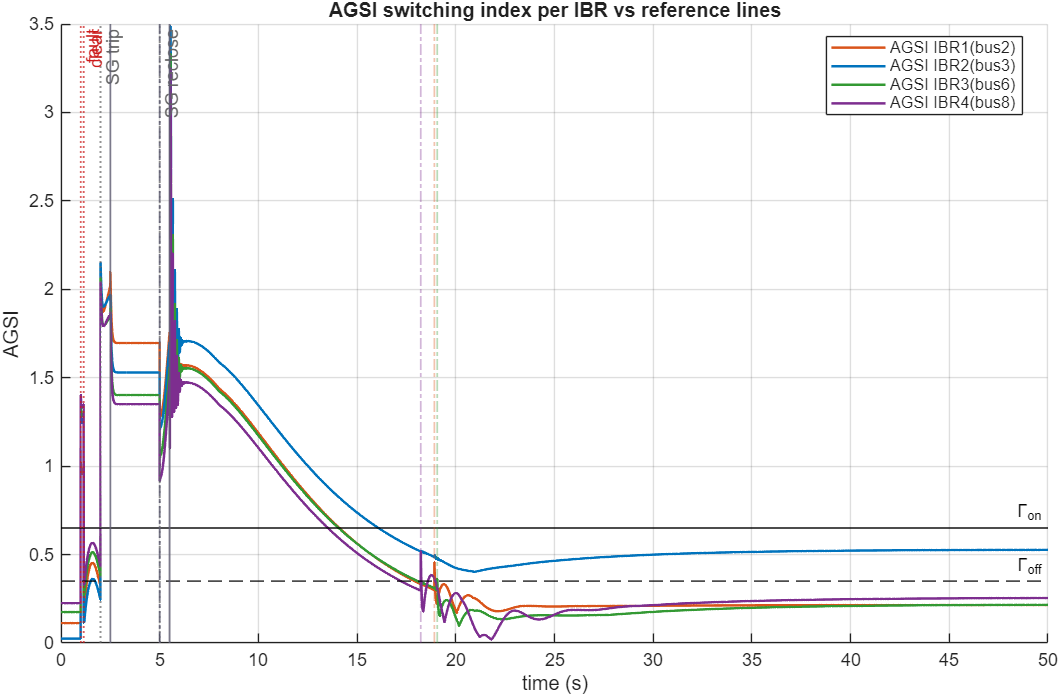
\includegraphics[width=0.8\linewidth]{figures/switch_ieee14/padiyar_switch_agsi.png}
\caption{IEEE 14-bus: AGSI++ per IBR (fault $Z_f{=}j0.1$ pu, then SG trip $2$ s, reclose $5$ s; $50$ s window).}
\end{figure}
\begin{figure}[H]\centering
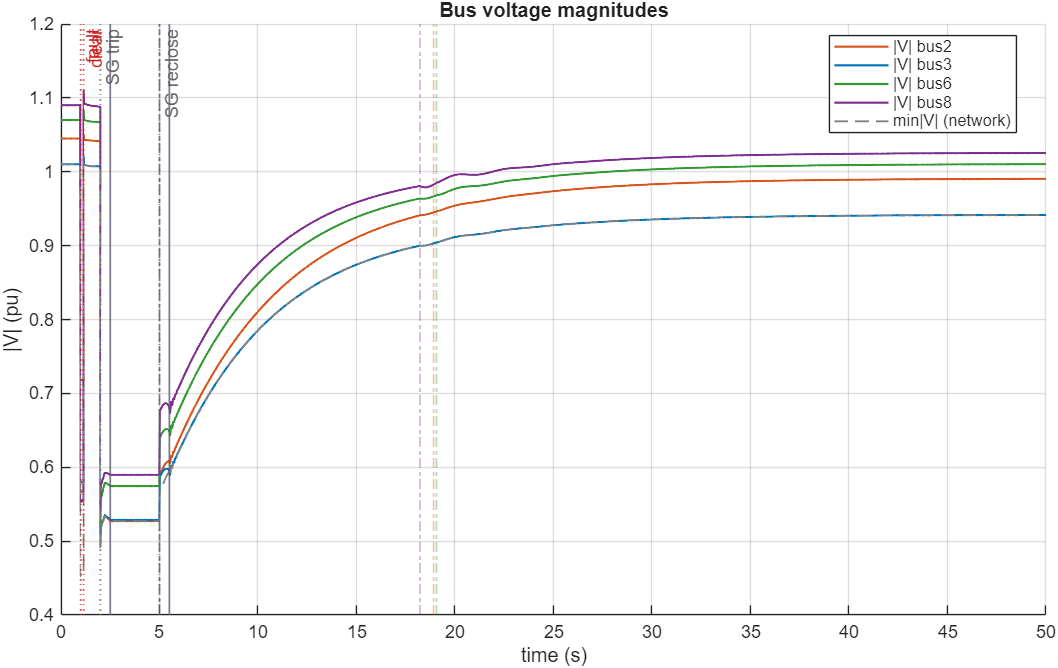
\includegraphics[width=0.8\linewidth]{figures/switch_ieee14/padiyar_switch_voltage.png}
\caption{IEEE 14-bus: bus voltages through the trip/reclose cycle.}
\end{figure}
\begin{figure}[H]\centering
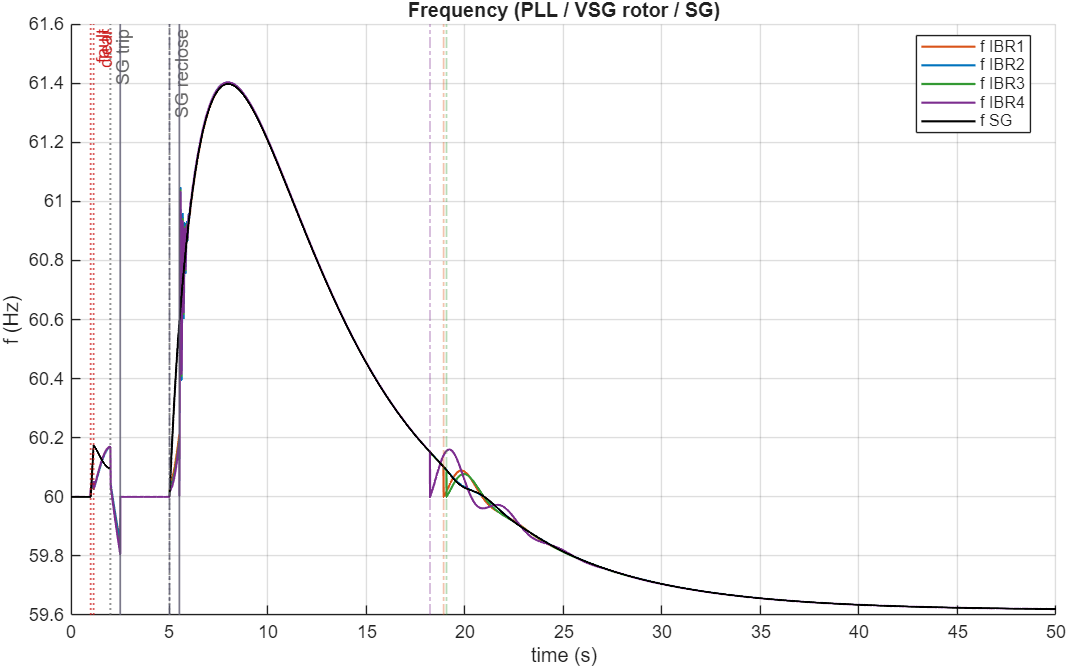
\includegraphics[width=0.8\linewidth]{figures/switch_ieee14/padiyar_switch_freq.png}
\caption{IEEE 14-bus: SG and IBR frequencies.}
\end{figure}
\begin{figure}[H]\centering
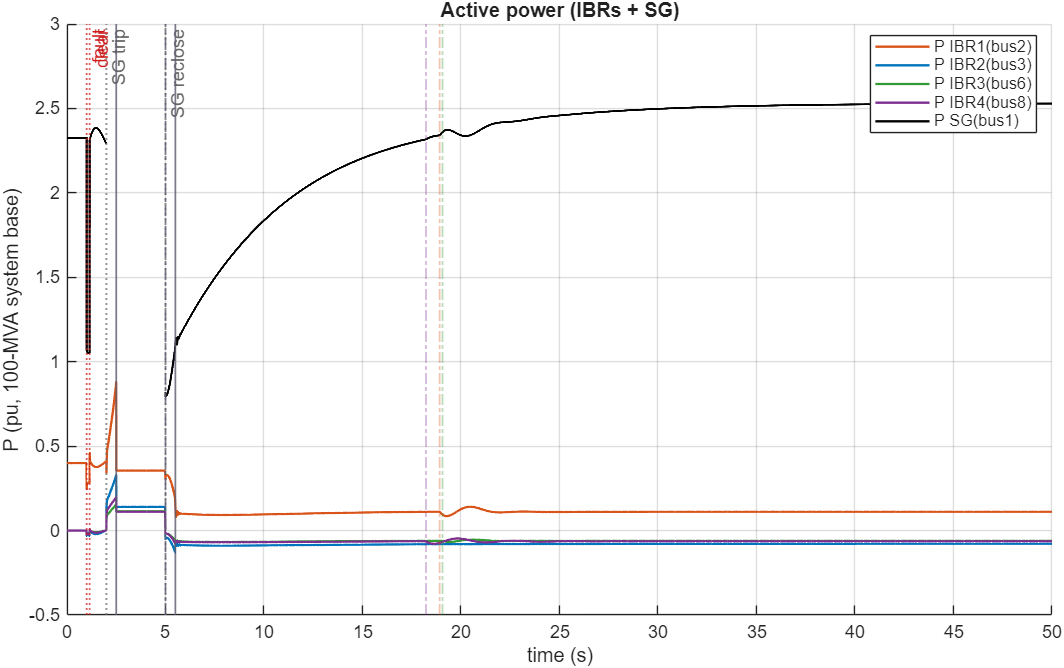
\includegraphics[width=0.8\linewidth]{figures/switch_ieee14/padiyar_switch_p.png}
\caption{IEEE 14-bus: active-power injections.}
\end{figure}

\subsection{Summary}
The two systems share an identical supervisor and event sequence but differ in outcome: the
Padiyar two-area operating point is small-signal unstable ($+0.058\ \mathrm{s^{-1}}$) and collapses
to all-GFM on a long run, whereas the meshed IEEE 14-bus operating point is stable and stays
bounded. AGSI++ keeps the index bounded and non-chattering in both cases.

\begin{thebibliography}{9}
\bibitem{eecon49en} EECON49-P4 (KMITL), ``A Bayesian Optimization-Based GFL/GFM Mode Switching
Strategy,'' The 49th Electrical Engineering Conference (EECON-49), 2026.
\bibitem{ding2025e} H. Ding \emph{et al.}, ``A novel design for switchable grid-following and
grid-forming control,'' \emph{IEEE Trans. Sustain. Energy}, vol.~16, no.~2, pp.~1301--1314, 2025.
\bibitem{liu2024e} P. Liu, X. Xie, and J. Shair, ``Adaptive hybrid grid-forming and grid-following
control of IBRs under varying SCRs,'' \emph{IEEE Trans. Power Electron.}, vol.~39, no.~6,
pp.~6603--6607, 2024.
\bibitem{gao2025e} X. Gao \emph{et al.}, ``Seamless switching method between grid-following and
grid-forming control,'' \emph{IEEE Trans. Ind. Appl.}, vol.~61, no.~1, pp.~597--606, 2025.
\bibitem{entsoe_rocof2} ENTSO-E, ``Rate of Change of Frequency (RoCoF) withstand capability,''
Network Code RfG implementation guidance document, 2018.
\end{thebibliography}

\end{document}
